\documentclass{ferseminar}
\student{Alen Murtić}
\voditelj{doc.~dr.~sc.~Damir Pintar}
\mjestodatum{Zagreb}{travanj}{2017}
\naslov{Data mining u sportu}
\begin{document}
\stvoripredstranice
\section{Uvod}

Proteklih 120 godina sport je polako postajao sve važniji element u svakodnevnom životu "običnih" ljudi. Iz krpenih lopti i dresova razvila se milijunska industrija koja pazi na svaki detalj kako bi sportaši postigli najveće moguće rezulate. Jedan od najvažnijih aspekata momčadskih sportova je donošenje odluka - treneri, sportski direktori, vlasnici i ostali djelatnici upravljaju velikim rizicima, a često nemaju potpune ili kvalitetne informacije, što je pomalo otužna činjenica u trenutnom informacijskom vremenu kada postoji toliko dostupnih podataka o sportu. Zato je stvorena posebna disciplina analize podataka u cilju poboljšanja kvalitete odluka koje sportski djelatnici moraju donositi.


Posebni dio ekosustava modernog sporta je klađenje. Sportsko klađenje mnogima je jedini razlog zašto prate sport. Kladionice također zarađuju milijune te su često veliki sponzori sportskih momčadi, npr. glavni sponzor 10 od 20 trenutnih članova engleske Premier lige su tvrtke koje nude igre na sreću. Svaki sportski fan koji se razumije u matematiku jednom je želio napraviti model predviđanja utakmica, no kladionice ne dopuštaju najuspješnijim igračima da se klade nakon određenog dobitka. Kladionice su uvijek na dobitku, a to postižu pažljivim promjenama koeficijenata uz pomoć naprednih algoritama. Očito je da one imaju veliku potrebu za analizom podataka kod promjene koeficijenata, detekcije najboljih igrača te detekcije namještenih sportskih dvoboja.


\textit{Data mining} (rudarenje podataka) je vrsta analize podataka čiji je cilj pronalaženje relevatnih informacija u podacima te iskorištenje istih za poboljšanje procesa donošenja odluka. Postoje dvije kategorije \textit{data miniga}: deskriptivna (otkrivajuća, opisna) te prediktivna (predviđajuća) analiza. Desktiptivna analiza u nestrukturiranim, prevelikim ili nejasnim podacima nalazi "skrivene" informacije te ih kranjem korisniku predstavlja u razumljivom obliku. Prediktivna pokušava naći pravilnosti u podacima te ih iskoristiti za predviđanje budućih. Ne postoji neka čvrsta granica između \textit{data mininga} i ostalih vrsta analiza podataka, no njegova najčvršća značajka je traženje i dubinska analiza.\cite{data}


Ovaj seminarski rad opisuje potrebu i korist \textit{data mininga} u sportu, postojeća rješenja te moguće nadogradnje. Fokusiran je na 3 vrlo različita timska sporta: košarku, nogomet i američki nogomet kako bi čitatelju prikazao što širi opus problema i ideja \textit{data mininga} u sportu.

\section{Potreba i korist data mininga u sportu}

Ovo poglavlje bavi se razlozima korištenja \textit{data mininga} u sportu prolazeći kroz 3 točke: izvorišne ideje te potrebe za deskriptivnom odnosno prediktivnom analizom. Važno je naglasiti da niti jedan sustav nije napravljen isključivo s ciljem zadovoljavanja neke od točaka, već je ovo jedan pokušaj klasifikacije područja kojima se \textit{data mining} u sportu bavi.

\subsection{Izvorišne ideje}
Većina ideja statističke analize u sportu dolazi iz baseballa, a za to postoje jasni razlozi:
\newline
1. baseball je sport s dugom tradicijom i velikom popularnošću, uvijek je bio profitabilan pa je privlačio mnogo novih ideja i pametnih ljudi. Bitna je i činjenica da je američka profesionalna liga MLB nastala spajanjem dvaju liga AL (American league) i NL (National league) koji su unutar MLB-a i dan danas donekle neovisne. Zbog toga su postojala dva "tržišta" za promociju sportske statistike.
\newline
2. legende sporta vrlo su važan element razgovora o baseballu, a budući da on ima turbulentnu i rasističku prošlost u SAD-u, postoji potreba za revizijom nekih dijelova iste.
\newline
3. njime dominira statistika, pogledom na detaljne rezultate od prije 100-tinjak godina može se razumjeti mnogo više o utakmicama nego kod ikojeg drugog sporta.\cite{mlb}
\newline

U engleskom jeziku postoji izraz \textit{sabermetrics} koji označava korištenje statistike u cilju razumijevanja baseballa (danas se koristi i u kontekstu ostalih sportova), a potječe od organizacije SABR (Society for American Baseball Research) nastale 1971. s ciljem elemenata tog sporta. Specifičnost organizacije je u tome da je sačinjena od novinara, bivših igrača, navijača, statističara i ostalih dionika sporta kako bi pružila što širi i točniji pogled na teme koje ju zanimaju.\cite{sabr}

Pravi rast data mininga u baseballu počinje kasnih 1990-ih i ranih 2000-ih, a najviše ga simboliziraju dvojica menadžera Billy Beane i Theo Epstein. Billy Beane je 1998. postao generalni menadžer (GM) Oakland Athleticsa, momčadi s prilično ograničenim budžetom u odnosu na protivnike. Beane je osmislio princip nazvan Moneyball, ideju kupovine podcijenjenih igrača u cilju optimizacije potrošnje novca. Igrače je evaluirao analitičkim metodama zasnovanim na matematici. Beane je godinama imao značajno bolje rezultate od mnogih skupljih momčadi, ali Oakland nije uspio osvojiti ligu. Theo Epstein je 2002. sa samo 28 godina postao GM Boston Red Soxa, kluba koji je 84
\newpage
\noindent godine bio bez trofeja prvaka. Samo 2 kasnije osvojili su naslov te to ponovili 2007.\cite{mlb}

Dominacija statistike u baseballu pomiješana s američkom zabranom tradicionalnog klađenja dovela je do značajnog razvoja amaterskog data mininga za \textit{fantasy baseball} (natjecanja u kojima sudionici biraju igrače, a birana močad s najboljom ukupnom statistikom pobjeđuje, a njezin autor dobiva nagradu). Vrhunski igrači često postaju zaposlenici profesionalnih klubova. Takva intelektualna širina zaslužna je za konstantan napredak \textit{data mininga} u baseballu.

Najveća godišnja konferencija sportske analitike je Sloan Sports Analytics Conference koja se svake godine održava na prestižnom sveučilištu MIT. \cite{Sloan}

\subsection{Potreba za desktiptivnom analizom}

Potreba za desktiptivnom analizom na bazičnoj razini prilično je očita - što više točnih informacija uvijek je bolje nego manje. No, budući da se ne možemo baviti svime, potrebno je identificirati ključne podatke koje želimo saznati.

\subsubsection{Raspodjela resursa}
Neizbježna činjenica svakodnevnog života ili upravljanja bilo kojom vrstom organizacije je ograničenost resursa, stoga ona očito vrijedi i za sportske klubove. Resurse koje klubovi imaju možemo podijeliti u 2 skupine: sportski i financijski. 
\newline
Kao financijski resurs razmatramo novac koji može biti siguran ili potencijalan, baš kao kod svakog poduzeća, no specifičnost sporta u odnosu na većinu drugih djelatnosti da postoji i potpuno siguran budući novac (npr. minimalne naknade za TV prava na kraju sezone). Raspodjela financijskih resursa u sportu bavi se vjerojatnošću postizanja određenih sportskih i/li financijskih ciljeva (npr. dividende vlasnicima, vraćanje kredita za stadion) uz investiciju financijskih u sportske resurse. Standardno pitanje ovog područja je "Isplati li se potrošiti 
iznos x na odštetu/plaću igrača y?".\cite{deloitte}
\newline
Sportski resursi vrlo su različiti od sporta do sporta, pa i između različitih liga istog sporta te navodim najčešće: dostupna minutaža, vrijeme treniranja, zdravlje igrača, dozvoljeni negativni rezultati do ostvarenja cilja, izbori na \textit{draftu} i sl. Oni mogu biti jednaki za sve momčadi (npr. dostupna minutaža), no kao što se vidi u popisu, uglavnom nisu, stoga je njihova analiza još izazovnija i zanimljivija. Dobar dio sportskih resursa nužno je opisivati i prediktivno kako bi saznali kvalitetnije informacije u cilju donošenja odluka.

\subsubsection{Analiza kvalitete i stila vlastite momčadi}
Izvorišna ideja deskriptivne analize je razumijevanje prednosti i mana vlastite momčadi kako bi treneri i/li sportski direktori imali točne informacije. Prvenstveno tražimo opis igrača u različitim ulogama kako bi otkrili alternativne strategije igranja ili kupovine novih igrača. Analiza kvalitete bavi se pretvorbom konkretnih podataka iz utakmica ili treninga u što jasniji opis, tj. pronalaženjem podataka koji ne bi bili uočeni.\cite{stats}

\subsubsection{Optimiranje strategije}
Optimiranje strategije izravno je poduprto znanjem dobivenim iz prethodne dvije točke. Umjesto da ovisimo o kreativnosti ljudi, optimiranje strategije daje ocjenu različitih strateških opcija te sugerira one koje sustav vidi kao najbolje.

\subsubsection{Analiza protivnika}
Kvalitetna analiza protivnika dug je i naporan proces koji bi trebalo pojednostaviti što je više moguće. Ona zapravo radi na sličan način kao optimiranje strategije, samo što traži najčešće protivnikove ideje i mane te njegov stil protiv momčadi kao naše. Nalazi se na granici opisa i predviđanja.

\subsubsection{Procjena slučajnosti}
Donošenje odluka u svakom sportu, a posebno nogometu, je često temeljeno na pitanju: učiniti promjenu ili ne? Treba li klub dati otkaz treneru, treba li trener zamijeniti napadača koji ne postiže golove nekoliko utakmica, promijeniti taktiku ili ne i sl.? Analitički pristup može dati odgovor koja je vjerojatnost da se dogodio negativan ishod utakmice uz igru koju je momčad pružila. Nekad je lako shvatiti da je protivnički vratar imao odličan dan i da je zato naš tim izgubio, ali u pravilu je teško objektivno procijeniti je li nešto slučajnost ili realnost, pogotovo ako se klub nalazi u zoni ispadanja. Npr. u sezoni 2011.-12. Wigan FC je imao katastrofalne rezultate prvih 29 kola engleske Premier lige, iako su očito igrali kvalitetno. No, klub nije dao otkaz treneru i sezonu je završio s 9 pobjeda iz 11 utakmica i spasio se od ispadanja. Takva strpljivost je rijetka, a dubinska analiza rezultata može dati odgovor isplati li se čekati.\cite{odds}

\subsection{Potrebe za prediktivnom analizom}

Osnovna potreba za prediktivnom analizom je činjenica da se u sportu uspjeh uglavnom ne procjenjuje trenutnim stanjem, nego rezultatima u nekoj budućnosti do koje tek treba doći. Zato je vrlo bitno imati predstavku kako će neki igrači doprinositi momčadi u budućnosti.
\newline
S druge strane - kladionice imaju konstantnu potrebu što točnijeg predviđanja rezultata utakmice i ostalih statistika. One su tvrtke koje vrijede milijune i rade s ukupnim milijunskim iznosima kod najatraktivnijih utakmica te im svaka mala optimizacija koeficijenata može donijeti ogromne iznose dodatnog novca.

\subsubsection{Predviđanje rezultata utakmica}
Predviđanje rezultata utakmica idejno je osnovni, a izvedbeno najteži dio prediktivne analize. Ti podaci bitni su i kladionicama, kako bi povećale zaradu i klubovima, za što informiranije planiranje sezone. Razvijene su različite tehnike predviđanja rezultata, od standardnih 3-klasnih klasifikatora (pobjeda, poraz, neriješeno) do vremenski ovisnih Markovljevih lanaca, posebno popularnih u nogometu.\cite{pred}

\subsubsection{Kvaliteta igrača kroz godine te rizik ozljeda}
Klubovima najzanimljiviji aspekt prediktivne analize je predviđanje kvalitete igrača kroz godine. Kad bi savršeno znali kako će se igrač razvijati, ne bi bacali novce na skupe i beskorisne transfere. Tu se u obzir uzima i rizik ozljeda određenog igrača, mnogi veliki talenti propadnu zbog nesretnih zdravstvenih okolnosti. Ideja se provodi u stvarnost nekom vrstom regresije krivulje kvalitete s obzirom na bazu podataka iz prošlosti te sličnosti igrača s drugima (visina, težina, prethodne ozljede, brzina, stil igre, dosadašnja krivulja, itd.).\cite{tennis}

\subsubsection{Simulacija taktike}
Simulacija taktike zanimljiva je ideja rješavanja donošenja odluka unutar utakmica, ona se oslanja na analizu protivnika, no njezina je bit predvidjeti kako bi protivnik reagirao kod određenog rezultata, koju će momčad izabrati i slično. Simulacija taktike izuzetno je bitna u nogometu zbog postojanja samo 3 zamjene, momčad koju trener odabere bi mogla biti što raznovrsnija kako bi odgovorila na različite mogućnosti protivnika, a onda kasnije uvoditi specijalizirane zamjene kod neke od situacija.

\section{Postojeća rješenja}

Tri navedena sporta odabrana su zbog njihove potpuno različite prirode - američki nogomet je situacijski sport na velikom terenu, sport u kojem se znanje odlučno štiti, a sve igrače teško je pratiti, nogomet nema čvrsto definiran tijek, u njemu je moguće, smisleno i korisno pratiti igrače, a košarka je stilom između njih, igra se na malom terenu, a može se pratiti još više stvari nego u nogometu.

Za sva tri (i druge sportove) u zadnje vrijeme karakteristično je praćenje bioloških podataka igrača u cilju prevencije nepotrebnih ozljeda. Ideja je relativno jasna: u slučaju da je igrač previše umoran, rizik od ozljeda raste nekoliko puta te je takve situacije poželjno izbjeći. Najrazvijenije je u košarci, tj. NBA-u gdje se čak počinje voditi rasprava smiju li klubovi tako narušavati privatnost igrača. \cite{bio}

\subsection{Košarka}

\subsubsection{Analiza kvalitete šuta} 
Najbitniji element košarke je postizanje poena, a kako šutevi za 1, 2 i 3 poena nemaju jednaku vrijednost, smišljene su nova mjere, EFG (\textit{effective field goal percentage}) i TS\% (\textit{true shooting percentage}). One, iako kvalitetne, ne opisuju do kraja stvarnost. Pucati trice točno s linije iz kornera (kuteva terena) nije isto kao pucati trice s linije ravno ispred koša. To su momčadi uočile već sredinom 1980.-ih, no nisu počele iskorištavati do iza 2010. \cite{corner3s} No, nije svaki šut svakog igrača jednak. Osim što gledamo poziciju na terenu, cilj je otkriti najbolje zone šuta za svakog igrača te najbolje šuteve općenito. A to su otvorene trice, zato što je njihova vrijednost puno veća te šutevi pored koša jer se lako realiziraju. Donekle solidan tricaš (daleko od elitnog) puca ~35\%, a da bi istu vrijednost postigao dvicama, mora gađati 3*0.35=2*x => x = 52.5\%. Posebno su grozne duge dvice, čija je preciznost samo malo bolja od trica, a donose samo dva poena. Zato momčadi moraju forsirati trice. \cite{NBAshots} Najdalje je u implementaciji tog principa otišao generalni menadžer Houston Rocketsa Daryl Morey čiji je cilj odigrati jednu utakmicu u kojoj će njegova momčad pucati samo trice i polaganja. Na slici 1 može se vidjeti jedan graf šuteva.

\begin{figure}[htb]
	\centering
	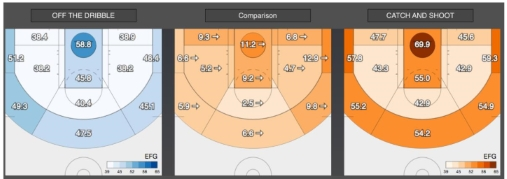
\includegraphics[]{img/shots.jpg}
	\caption{Prikaz kvalitete šuta iz rada \cite{NBAshots}}
	\label{fig:shots}
\end{figure}

\subsubsection{Predviđanje kvalitete igrača na \textit{draftu}}
Košarka je jedinstven momčadski sport po tome što jedna superzvijezda s 4 loša igrača momčadi doprinosi više nego 5 solidnih te je stoga cilj svakog NBA kluba pronaći sljedeću superzvijezdu. Budući da igrači u ligu dolaze \textit{draftom} (slijednim pravom na izbor 1 igrača od najgoreg do najboljeg kluba prošle sezone), cilj svakog kluba je odabrati najboljeg dostupnog igrača ili napraviti zamjenu za bolji izbor dajući neke trenutne ili buduće resurse. To je veliki izazov za svakog matematički pismenog pratitelja sporta te postoje doslovno stotine modela za \textit{draft}, a poveznica prikazuje neke najpoznatije. \cite{models}

Njihova ideja je po prirodi jednostavna: uzeti što više dostupnih podataka o igraču te temeljem prethodnih godina naći najvjerojatniju projekciju njegove karijere, no izvedbe su prilično komplicirane i relativno netočne. Uvijek se postavlja pitanje koliko utjecaja na ishod karijere pojedinca ima okolina, a koliko sam igrač.

\subsection{Nogomet}

Nogomet je globalni sport te stoga postoji velik broj ljudi koji žele pronaći napredna analitička rješenja za izazove s kojima se nogometne momčadi susreću. Njihovi pristupi kreću od metodičnog analiziranja taktike uz popratnu statistiku (npr. spielverlagerung.de), a završavaju u potpuno numeričkom opisu nogometa koji nisu baš previše popularni. \cite{soccAn} Zato ćemo opisati 2 različita pristupa nogometnom \textit{data miningu} - računalna reprezentacija nogometa utakmica te skautiranje Football Managerom.

Daleko najpopularnija vrsta analitike u nogometu koji se čak koristi i u nekim HNL klubovima je praćenje utakmice kamerama te modeliranje događaja (trčanja igrača, dodavanja) u ljudima čitljivom obliku. Njome se bave tvrtke poput OptaSports ili Squawka Football, a rezultat takve analitike vidi se na slici ispod. Ideja takvog pristupa je dati trenerima ili sportskim direktorima što više podataka kako bi oni informirano donosili odluke. 

\begin{figure}[htb]
	\centering
	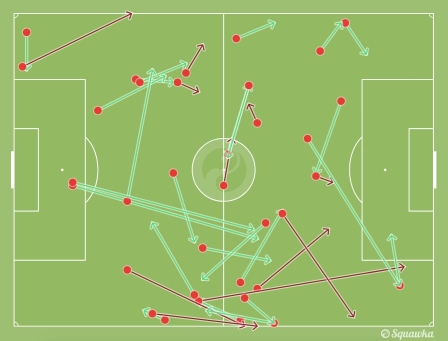
\includegraphics[]{img/squaka.jpg}
	\caption{Slika prikazana u sustavu Squaka Footballa \cite{NBAshots}}
	\label{fig:shots}
\end{figure}

Jedna od najzanimljivijih metoda nogometnog \textit{data mininga} je korištenje baze podataka koju ima Football Manager (FM). Na njoj svake godine rade stotine novinara iz mnogo različitih zemalja kako bi bila što točnija za svaku od liga te tako imala što više kupaca. I ne, ne koristi se FM bazom podataka samo " nogometna sirotinja", već i najuspješniji svjetski klubovi. \cite{FM} Budući da na njoj rade lokalni novinari, ona sadrži podatke koje strani skauti možda ne razumiju, neku vrstu institucionalnog znanja. Postoji još i dodatna razina korištenja FM-a u kojoj se temeljem empirijski dokazanih podataka i popisa ljudi koji su radili na podacima pojedine zemlje može analizirati koje su nacionalnosti precijenjene, a koje podcijenjene.

Zašto je FM toliko koristan za \textit{data mining} u sportu? Razlog je jednostavan, ne postoji potreba za apstrakcijom podataka, sve su ih u brojke pretvorili stvarni ljudi, a strastveni igrači ih godinama koriste. 

\subsection{Američki nogomet}
Američki nogomet specifičan je sport zbog toga što se igra prekida nakon svake akcije te postoji mogućnost zamjene igrača nakon istih. Na terenu svaka momčad ima jedanaestoricu od kojih samo jedan ili dvoje igraju loptom u pojedinoj napadačkoj akciji (osim kod jako, jako rijetkih dodavanja unazad) zato što je dozvoljeno samo 1 dodavanje prema naprijed, no svi ostali trče ili blokiraju kako se otvorilo što više prostora za igrača s loptom. Sve akcije su tajne unutar momčadi te stoga ne postoji mnogo javnih modela za američki nogomet. Ono što znamo je da neki klubovi koriste \textit{data mining} jer se u zadnje vrijeme ruši mnogo starih neefikasnih principa (držanja osrednjih veterana,
\newpage\noindent visokih odabira trkača na \textit{draftu}, favoriziranje trčanja u odnosu na dodavanje) te dodaju neki novi (kasnije navedeni).

Iako je većina \textit{data mininga} u NFL-u tajna, jedna od najnaprednijih sportskih \textit{data mining} stranica je specijalizirana za američki nogomet, Pro Football Focus. Također postoje doslovno stotine stranica koje se bave fantasy footballom, dozvoljenim oblikom klađenja u Americi.
\newline
Opišimo kako je svaki od starih principa unaprijeđen te koji su novi principi:
\begin{itemize}
	\item Držanje osrednjih veterana \cite{ringer_age}
	\newline
	Budući da u NFL-u postoji maksimalni iznos novaca koje momčadi smiju potrošiti, da bi vrhunski klubovi ostajali pri vrhu, moraju povremeno puštati osrednje starije igrače da odu te plaćati samo najbolje. Specifičnost lige je da u slučaju odlaska najboljih igrača klubovi dobiju kompenzacijske odabire na \textit{draftu}. Dok tog ograničenja nije bilo (prije 1990.-te), klubovi su zadržavali sve korisne igrače. No, sada ne mogu, te moraju postati praktički tvornice igrača kako bi ostali u vrhu.
	\item Visoki odabir trkača na \textit{draftu} \cite{RBs}
	\newline
	Budući da je liga počela favorizirati dodavanja te da je skauting bolji nego ikada, u NFL-u se visokim izborima više ne isplati odabirati trkače zato što ih se lako može naći vrlo jeftino, isključujući vrhunske talente. Trkači imaju kraće karijere nego druge napadačke pozicije zbog izloženosti ozljedama te je stoga i vremenska vrijednost takvog odabira mala. To se jasno vidi na slici 3 koja prikazuje broj osvojenih jardi trkača i hvatača prema životnoj dobi. \cite{RBs2}
	
	\begin{figure}[htb]
		\centering
		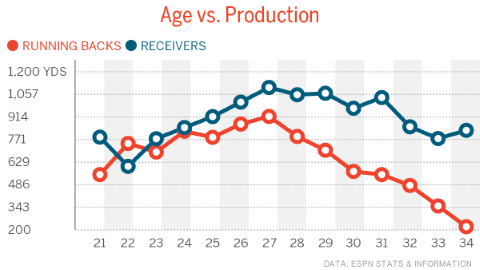
\includegraphics[]{img/rbs.png}
		\caption{Broj osvojenih jardi trkača i hvatača prema životnoj dobi, ESPN.com}
		\label{fig:shots}
	\end{figure}
	\newpage
	\item Favoriziranje trčanja u odnosu na dodavanje
	\newline
	Zbog novih pravila koja zaštićuju zdravlje igrača, NFL momčadima je sve lakše izvoditi uspješna dodavanja koja su gotovo uvijek dalja nego uspješne trke te se stoga očito osjeti velika promjena u stilu igre. \cite{RBs}
\end{itemize}
Osim razbijanja starih principa, formirani su i neki novi od kojih spomenimo dva najbitnija:
\begin{itemize}
	\item Shvaćanje vrijednosti napadačke linije
	\newline
	Napadačka linija je 5 igrača u sredini svake napadačke akcije koji ne smiju napredovati s loptom u rukama (niti je hvatati) te su zato dugo vremena bili potcijenjeni. Njihov zadatak je čuvanje dodavača ili trkača od protivničke obrane. Međutim, budući da je dodavač najbitniji i najplaćeniji igrač svakog kluba, logično je da ga se mora što bolje zaštiti, pa makar i pod cijenu slabljenja drugih dijelova momčadi. Empirijski je dokazano da klubovi koji više resursa utroše u ofenzivnu liniju imaju bolje rezultate dodavanja. \cite{OL}
	\item Izbacivanje srednje dugih dodavanja \cite{Deep}
	\newline
	Nešto potpuno novo u NFL-u, idejno preuzeto iz košarke (pucanje mnogo trica), je izbacivanje srednje dugih dodavanja u korist dugačkih. Statistika pokazuje da su srednje duga dodavanja slično uspješna/neuspješna, a duga daju veću korist. Duga dodavanja imaju veću varijancu te se tako mogu nadoknaditi veliki zaostaci, baš kao New England Patriotsi u Super Bowlu ove godine. \cite{NEP}
\end{itemize}

\section{Nove mogućnosti}

Dvije nove mogućnosti \textit{data mininga} u sportu koje su relativno slabo istražene, koliko je poznato (možda postoje neki privatni sustavi), su simulacija utakmica i \textit{text mining} izvještaja djelatnika klubova, ponajprije skauta.

Simulacija utakmica zanimljiva je ideja predviđanja rezultata. Statistika može dati vjerojatnosti pojedinih događaja i rezultata, no simulacije mogu dati točnije vjerojatnosti jer mogu uzeti u obzir neočekivane parametre, npr. izglede da se dogodi isključenje nekog igrača u nogometu koji kao rezultat simulacije mogu biti točnije nego \textit{a priori} vrijednosti jer postoji nešto što \textit{a priori} zanemarujemo. Postoje različite vrste simulatora, a najpoznatiji su sportske igrice (npr. već spomenuti Football Manager ili NBA 2k) ili stranice poput whatifsports.com koje predviđaju rezultate utakmica vremenski razdvojenih momčadi. Teško je dati neki detaljniji uvid u simulaciju bez dulje razrade sustava, već samo valja napomenuti da se u drugim područjima to zove Monte-Carlo metoda. \cite{monte}  

\textit{Text mining} je postupak pronalaženja novog znanja iz teksta (za razliku od information retrievala koji se zavi vađenjem već zapisanog znanja). \cite{textmin} Temeljen je na činjenici da je ljudsko znanje uglavnom sadržano u tekstualnoj formi te da ga se zato vrijedi analizirati. U sportu su posebno važni opisi igrača koje daju klupski djelatnici (skauti) koji u obzir mogu uzeti daleko više stvari nego računalo, no ne mogu ih obraditi niti na približnoj razini računala. Ideja takvog pristupa je naći kvalitetu, prednosti i mane pojedinog skauta te ih zapisati kao neku funkciju koja preslikava nove izvještaje u vjerojatnosti ishoda. \cite{textminNHL} Najveći nedostatak cijelog procesa je činjenica da se svi ljudi mijenjaju s vremenom, pa je teško odrediti definitivna preslikavanja izvještaja i predviđanja.

Najveći nedostatak svakog oblika obrade prirodnog jezika (NLP) je kombinatorna eksplozija sadržaja koji se može izreći vokabularom što rezultira ne baš sjajnom točnošću rezultata. Specifičnost zašto je \textit{text mining} jako zanimljiv izbor za sport je činjenica da vokabular sporta nije jako širok pa bi se čak mogli napraviti kvalitetni i primjenjivi nadzirani modeli uz znanje eksperata.

\section{Zaključak}

Ovaj seminar dao je prikaz tematike kojom se bavi \textit{data mining} u sportu kroz tri različite perspektive triju sportova. Kako bi u potpunosti razumjeli analitički pristup, potrebno je razumjeti njegovu prošlost (tj. postupni nastanak) te potrebe i probleme koje algoritmi trebaju zadovoljiti. Oni mogu biti deskriptivni i prediktivni. Deskriptivni su: raspodjela resursa koji mogu biti sportski (minute, prava na izbor igrača) i financijski, analiza kvalitete i stila vlastite momčadi u cilju boljeg razumijevanja situacije, optimiranje strategije da bi npr. igrali svi najbolji igrači, analiza protivnika te procjena koliko su rezultati slučajni, a koliko realni. S druge strane, prediktivni problemi su: predviđanje rezultata utakmica, kvalitete igrača kroz godine (kao i njegov rizik ozljeda) te simulacija taktike u utakmici.

Nakon toga, seminar donosi rješenja tih problema u košarci, nogometu i američkom nogometu. U košarci možemo analizirati npr. kvalitetu šuta i budućnost igrača na \textit{draftu}, u nogometu možemo pratiti igrače i stil momčadi, a u američkom nogometu ne navodi konkretna rješenja zbog "tajnosti" profesionalnih klubova nego očite pomake koje je \textit{data mining} donio u odlučivanju.

Zatim prikazuje dva moguća buduća rješenja - simulacija samih utakmica i \textit{text mining} analiza predviđanja djelatnika klubova budući da je većina podataka kojima ljudi barataju zapisana u tekstualnom obliku.

Neupitno je da sve sportske momčadi žele što efikasnije raspolagati svojim resursima i donositi što bolje odluke. Zbog toga, očito je da kvalitetan \textit{data mining} u sportu ima svijetlu budućnost.

\dodajliteraturu{bazaLiterature}
\section{Sažetak}

Seminar prikazuje \textit{data mining} u sportu objašnjavajući njegovu povijest, sadašnja rješenja te moguće nove ideje. Najprije se navode problemi koje \textit{data mining} može rješavati, oni su, između ostaloga: raspodjela resursa, analiza kvalitete momčadi, optimiranje strategije, analiza protivnika, procjena slučajnosti, predviđanje rezultata utakmica te kvalitete igrača, kao i simulacija taktike.

Seminar zatim iznosi neka od rješenja u 3 vrlo različita sporta - košarka, nogomet i američki nogomet ne ulazeći u implementacijske detalje pojedinih algoritama i principa. Najvažniji algoritmi tiču se analize kvalitete šuta u košarci, predviđanja karijere igrača u košarci i nogometu, praćenje igrača u nogometu te princip raspodjele resursa u američkom nogometu.

Sljedeće poglavlje predstavlja neke od ideja za nove mogućnosti s velikim potencijalom, neke od njih su analitičari već dotaknuli, posebno ističući ideju tekstualne analize izvještaja djelatnika klubova i njihovih predviđanja kvalitete igrača.

Sve kulminira zaključkom koji donosi kratki osvrt na seminar te potvrđuje ideju da \textit{data mining} u sportu ima svijetlu budućnost.

\end{document}
